\section{Model}
\label{sec:model}
We seek to allocate the outbound link bandwidth among client VMs, to ensure:  

{\bf 1. Congestion Freedom:}  The sum of the allocated bandwidths does not
exceed the outbound link bandwidth.

{\bf 2. Strong Fair Allocation: } The bandwidth is divided among clients in
proportion to their weights, not exceeding their demand. Leftover bandwidth is
dividied proportionally.

\begin{figure*}[t]
\center
\subfigure[Standard Fair queuing model]
{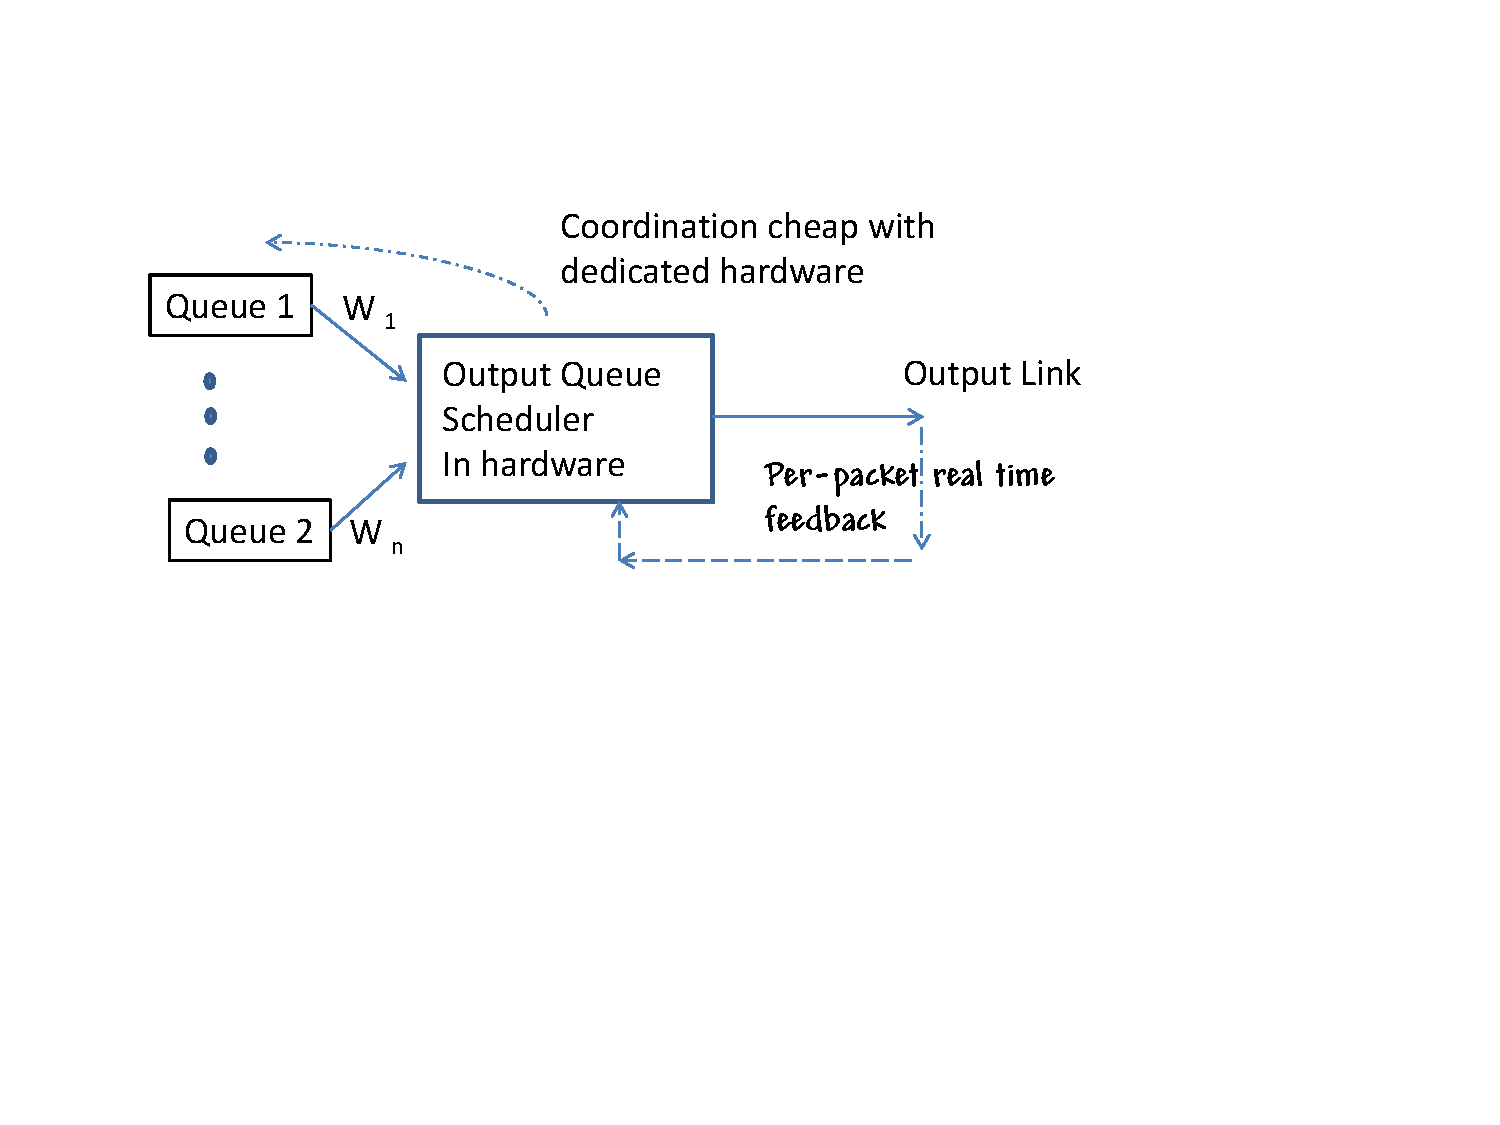
\includegraphics[width=0.3\textwidth,trim=6mm 90mm 20mm 10mm]{figures/standardqosmodel}
\label{fig:qosmodel}
}
\subfigure[VM Fair Queuing model]
{
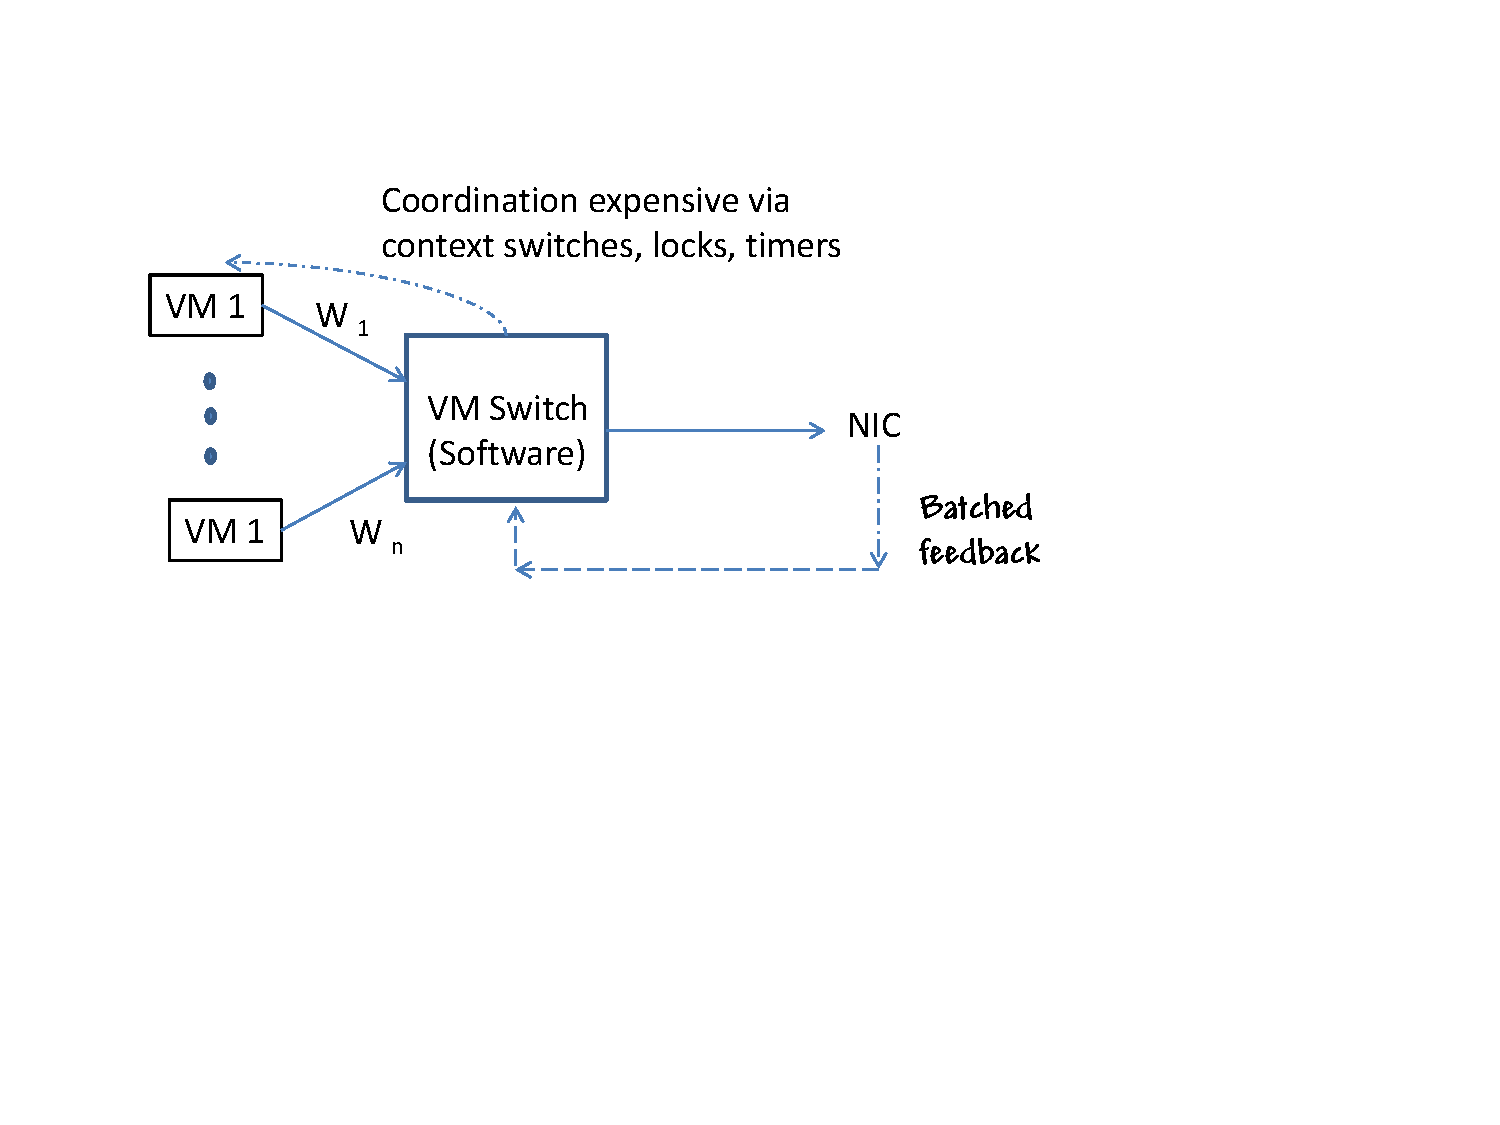
\includegraphics[width=0.3\textwidth, trim=6mm 90mm 20mm 10mm]{figures/vmqosmodel}
\label{fig:vmqosmodel}
}
\subfigure[Macro-Micro scheduler model]
{
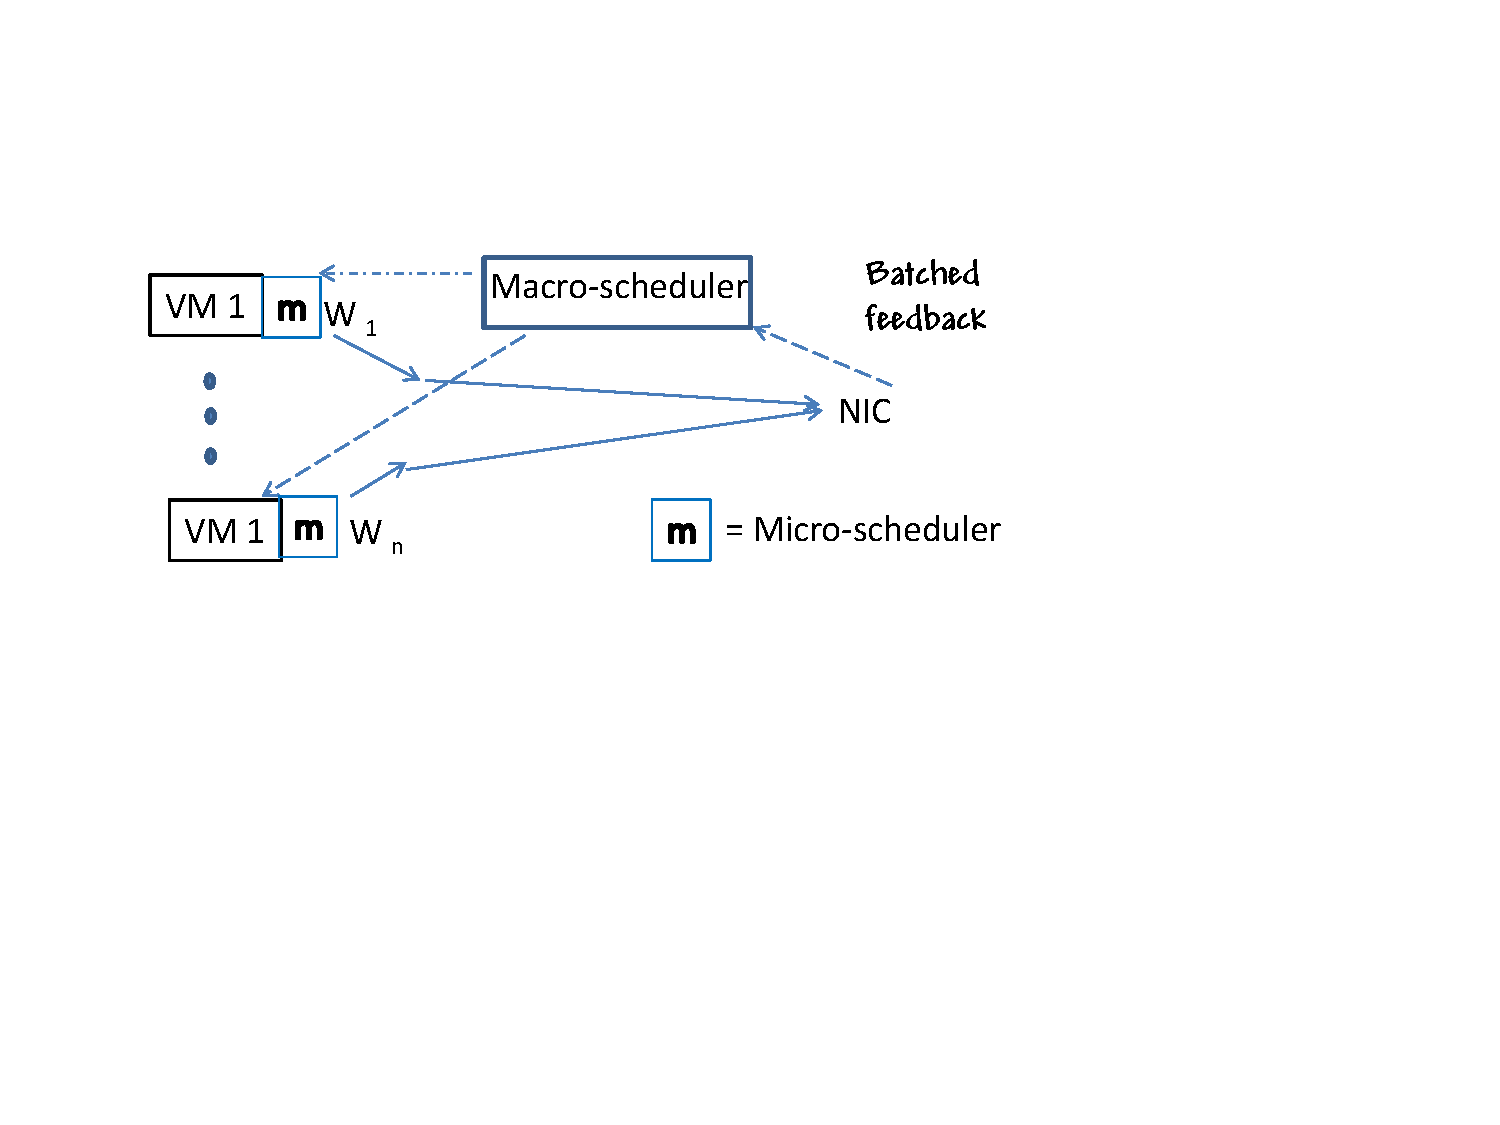
\includegraphics[width=0.3\textwidth, trim=6mm 90mm 20mm 10mm]{figures/macroschedule}
\label{fig:macroscheduler}
}
\vspace{-0.2em}
\caption{Scheduling models}
\label{fig:sched_mod}
\vspace{-0.5em}
\end{figure*}

Classical fair queuing model (Figure~\ref{fig:qosmodel}) used by algorithms such
as DRR~\cite{drr} and WF2Q~\cite{wf2q} make two implicit assumptions. First,
after packet transmission the link alerts the hardware scheduler who chooses the
next packet to transmit. Second, the scheduler is able to keep up with link
speed.  Both assumptions are reasonable for hardware routers.

However, in our model  (Figure~\ref{fig:vmqosmodel}) the feedback loop between
link and scheduler is batched.  Modern NICs use mechanisms like Large Send
Offload (LSO) to minimize overhead, so they can only generate one send-complete
notification for a group of packets.  Without per-packet feedback, a DRR
software implementation will receive transmit completion notifications in
bursts.  Besides causing transmit jitter, the bursts can be far apart with
respect to packet arrivals, causing packets to be dropped. Second, even if the
NIC could invoke the scheduler on a per-packet basis, the cost of running the
scheduler after every packet departure will be prohibitive. It typically takes
at least one full core to saturate a 40Gbps link. 

Implementations of weighted fair queuing algorithms like QFQ~\cite{qfq} solve
this problem by using technologies such as DPDK~\cite{dpdk} or
NetMap~\cite{netmap}, that allow them to bypass the NIC batching.  This is not
feasible in our scenario. For fine-grained scheduling, they also require more
CPU cycles than we can afford to spend.
 
We must also consider another subtle issue.  The software entity that
schedules packets from the queues must ensure that packets are en-queued to the
NIC's transmit buffer in the same order that they are de-queued from VSwitch
queues.  

There are two options to achieve this. First, the software could use a handle to
the NIC's transmit buffer.  This requires strong coordination between the
software module and the NIC's driver.  This is not feasible for a software
implementation on top of a hardware abstraction layer (e.g. NDIS in Windows).
in a general-purpose OS that must work across many NIC vendors A second
alternative is to make the software entity single-threaded so that each packet
is processed sequentially through the entire software stack from VSwitch to NIC
using a single processor. This is not scalable at multi-gigabit speeds.
Additionally, having to process packets on a single thread forces packets that
were processed on different processors to be then processed on a different
single processor, leading to cache misses which increase latency.

Our solution is to divide the scheduler into two entities as shown in
Figure~\ref{fig:macroscheduler}.   The macroscheduler runs only every $T$
seconds and hence can run on a single thread.   The microschedulers, by
contrast, run on every packet based on tokens allocated by the microscheduler.   

While this model reduces overhead it has obvious drawbacks because allocations
can only occur in units of $T$ seconds.   Thus we have two measures $T_{inc}$
which defines the worst case time for a VM to increase to its guaranteed
bandwidth, and $T_{dec}$ which is the worst case time after a VM decreses below
its allocation till the unused bandwidth is distributed to all active VMs. 
